\documentclass[a4paper,14pt]{extarticle}
\usepackage[english,russian]{babel}
\usepackage[cache=false]{minted}
\usepackage{fontspec}
\usepackage{indentfirst}
\usepackage{listings}
\usepackage{color}
\usepackage{caption}
\usepackage{amsmath}
\usepackage{hyperref}
\usepackage{graphicx}
\usepackage[%
    left=20mm,%
    right=10mm,%
    top=20mm,%
    bottom=20mm,%
]{geometry}%
\usepackage{titlesec}


\setmainfont{PT Astra Serif}

\hypersetup{
    colorlinks=true,
    linkcolor=black,
    filecolor=magenta,
    urlcolor=cyan,
    pdftitle={Лабораторная работа №4},
    pdfpagemode=FullScreen,
}

\newcommand{\hlink}[2]{\href{#1}{\color{blue}\underline{#2}}}
\graphicspath{ {./images/} }

\setmonofont[Scale=0.8]{JetBrains Mono}
\setminted{frame=lines, framesep=3mm, fontsize=\small}
\usemintedstyle{vs}

\titleformat{\section}
{\normalfont\bfseries}{}{0pt}{Упражнение \thesection.\;}

\titleformat{\subsection}
{\normalfont\bfseries}{}{0pt}{Задание \thesubsection.\;}

\numberwithin{figure}{section}

\begin{document}

\begin{titlepage}
    \vspace{0pt plus2fill}
    \noindent

    \vspace{0pt plus6fill}
    \begin{center}
        \textbf{\large{Санкт-Петербургский национальный исследовательский университет информационных
                технологий, механики и оптики}}

        \vspace{0pt plus2fill}
        \textbf{\Large{ЛАБОРАТОРНАЯ РАБОТА №5}}

        \vspace{0pt plus2fill}
        \textbf{\large{Создание и использование массивов}}
    \end{center}

    \vspace{0pt plus8fill}
    \begin{flushright}
        Студент: \\
        \textit{Швалов Даниил Андреевич}

        \textit{Факультет ИКТ}

        Группа: \textit{К32211}

        Преподаватель: \\
        \textit{Иванов Сергей Евгеньевич}
    \end{flushright}

    \vspace{0pt plus4fill}
    \begin{center}
        {Санкт-Петербург~--- 2023}
    \end{center}
\end{titlepage}

\section{Работа с массивом размерного типа данных}

В первой части задания необходимо создать массив, занулить все четные элементы и вывести элементы массива в стандартный вывод:
\inputminted{csharp}{../Loop/Loop/Program.cs}

\begin{figure}[H]
    \centering
    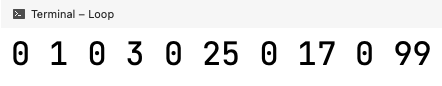
\includegraphics[width=0.5\textwidth]{images/task-1-1.png}
    \caption{Вывод программы}
\end{figure}

Во второй части задания необходимо считать массив со стандартного входа и вывести значения введенного массива в стандартный вывод:
\inputminted{csharp}{../Loop/Loop/Program1.cs}

\begin{figure}[H]
    \centering
    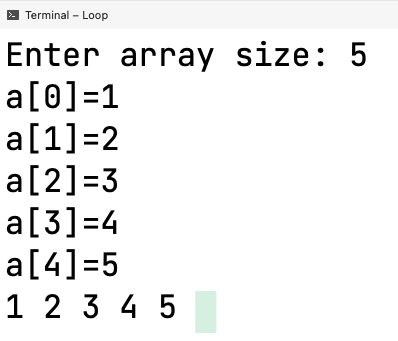
\includegraphics[width=0.5\textwidth]{images/task-1-2.png}
    \caption{Пример работы программы}
\end{figure}

\section{Перемножение матриц}

Сначала реализуем перемножение матриц на заранее заданных данных:
\inputminted{csharp}{../MatrixMultiply/MatrixMultiply/MatrixMultiply.cs}

\begin{figure}[H]
    \centering
    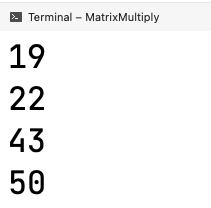
\includegraphics[width=0.5\textwidth]{images/task-2-1.png}
    \caption{Результат работы программы}
\end{figure}

Выделим вывод массива \texttt{result} в отдельную функцию \texttt{Output}:
\inputminted{csharp}{../MatrixMultiply/MatrixMultiply/MatrixMultiply1.cs}

\begin{figure}[H]
    \centering
    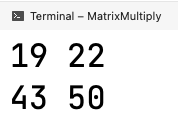
\includegraphics[width=0.5\textwidth]{images/task-2-2.png}
    \caption{Результат работы программы}
\end{figure}

Выделим расчет значений массива в отдельную функцию \texttt{Multiply}:
\inputminted{csharp}{../MatrixMultiply/MatrixMultiply/MatrixMultiply2.cs}

Изменим тело фукнции \texttt{Multiply}, заменив текущее решение на решение с циклом \texttt{for}:
\inputminted{csharp}{../MatrixMultiply/MatrixMultiply/MatrixMultiply3.cs}

Добавим возможность считывания матриц:
\inputminted{csharp}{../MatrixMultiply/MatrixMultiply/MatrixMultiply4.cs}

\begin{figure}[H]
    \centering
    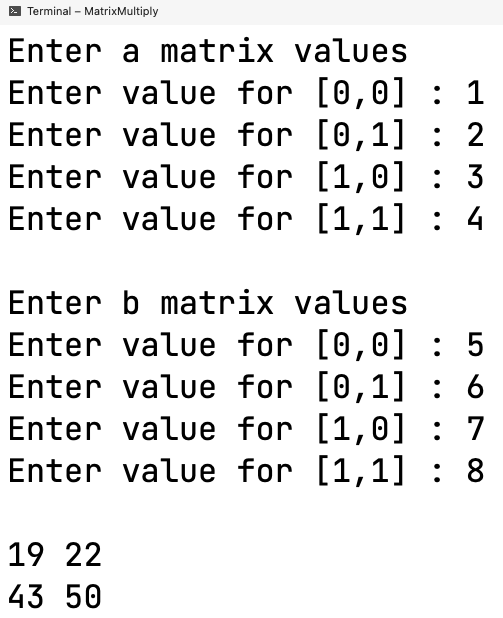
\includegraphics[width=0.5\textwidth]{images/task-2-3.png}
    \caption{Результат работы программы}
\end{figure}

\section{Обработка данных массива}

Каждую запрашиваемую функциональность реализуем в отдельных функциях. Исходный код программы представлен на следующем листинге:

\inputminted{csharp}{../MatrixOperations/MatrixOperations/Program.cs}

\begin{figure}[H]
    \centering
    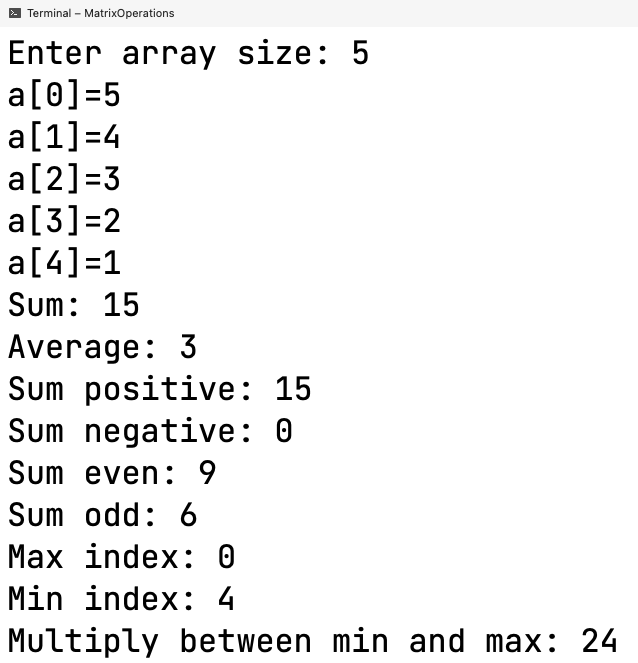
\includegraphics[width=0.5\textwidth]{images/task-3.png}
    \caption{Пример работы программы}
\end{figure}

\end{document}
